\section{Options}

\subsection*{4.1.1 European Vanilla Options}

Holder of European call, payoff
\[\phi(T) = \max(0,S_T-X)\]
Profit
\[\phi(T) -c/d_{0,T}\]

Holder of European put, payoff
\[\phi(T) = \max(0,X-S_T)\]
Profit
\[\phi(T) -p/d_{0,T}\]

\subsection*{4.2.1 Options and Underliers}
\begin{itemize}
    \item Short Call, Long Asset (Buy-Write) (Covered Call)
    \item Long Put, Long Asset (Protective Put)
\end{itemize}

\subsection*{4.2.2 Spreads}
Assume $X_i < X_j \Leftrightarrow i < j$
\begin{itemize}
    \item Bull Spread - Long Call $X_1$, Short Call $X_2$\\
    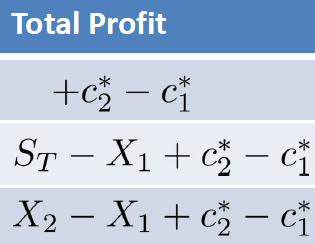
\includegraphics[width=0.2\linewidth]{contents/4.2.2.1.png}
    \item Bear Spread - Short Put $X_1$, Long Put $X_2$\\
    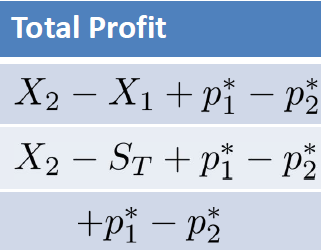
\includegraphics[width=0.2\linewidth]{contents/4.2.2.2.png}
    \item Box Spread - Combine Bull + Bear Spread, $PV=(X_2-X_1)d_{0,T}$
    \item Butterfly Spread - Long Call $X_1,X_3$, Short Call 2x $X_2$, $c_b=c_1+c_3-2c_2$\\
    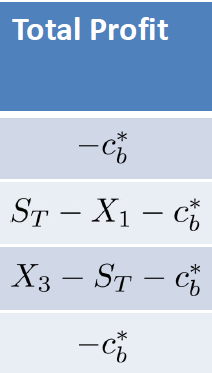
\includegraphics[width=0.1\linewidth]{contents/4.2.2.4.png}
\end{itemize}

\subsection*{4.2.3 Combination}
\begin{itemize}
    \item (Top) Straddle - Long Call, Long Put $X$
    \item Strip - Long Call, Long 2x Put $X$
    \item Strap - Long 2x Call, Long Put $X$
    \item Strangle - Long Call $X_2$, Long Put $X_1$
\end{itemize}
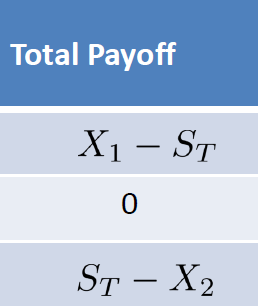
\includegraphics[width=0.1\linewidth]{contents/4.2.3.4.png}
